\documentclass[10pt,a4paper]{article}
\usepackage[utf8]{inputenc}
\usepackage[T1]{fontenc}
%\usepackage{stringenc} % for grffile
%\usepackage{ucs}
\usepackage{amsthm} %numéroter les questions
\usepackage[english]{babel}
\usepackage{datetime}
\usepackage{scrextend} %\footref{}
\usepackage[normalem]{ulem}
\usepackage{xspace} % typographie IN
\usepackage{hyperref}% hyperliens
\usepackage[all]{hypcap} %lien pointe en haut des figures
\usepackage[english]{varioref} %voir x p y
\usepackage{fancyhdr}% en têtes
%\input cyracc.def
\usepackage[]{graphicx} %include pictures
%\usepackage[encoding,inputencoding=utf8,filenameencoding=utf8]{grffile}
%\usepackage[extendedchars,inputencoding=latin1,filenameencoding=latin1]{grffile}
\usepackage[siunitx ]{circuitikz}
%\usepackage{gnuplottex}
\usepackage{ifthen}
\graphicspath{{./figures/}}
%\usepackage{array}
\usepackage{amsmath}
\usepackage[]{xcolor}
\usepackage{tikz}
\usepackage{tikz-timing}
\usetikzlibrary{scopes}
\usetikzlibrary{backgrounds}
\usepackage{listings}
\usepackage{enumitem}
\usepackage[top=1 in, bottom=1 in, left=1.3 in, right=1 in]{geometry} % Yeah, that's bad to play with margins
\usepackage[]{pdfpages}
\usepackage{pdflscape}
\usepackage[]{attachfile}
%\usepackage{colortbl}
%\usepackage{multirow}
\usepackage{booktabs}
\usepackage{makecell}
\usepackage[ ]{subfig}
%\usepackage{rotating}

\newcommand{\version}{v1.0.3}

%cyr
%\newcommand\textcyr[1]{{\fontencoding{OT2}\fontfamily{wncyr}\selectfont #1}}


\newboolean{corrige}
%\setboolean{corrige}{true}%corrigé
\setboolean{corrige}{false}% pas de corrigé

\newboolean{annexes}
%\setboolean{annexes}{true}%annexes
\setboolean{annexes}{false}% pas de annexes

\newboolean{mos}
%\setboolean{mos}{true}%annexes
\setboolean{mos}{false}% pas de annexes

\usepackage{aeguill} %guillemets

%% fancy header & foot
\pagestyle{fancy}
\lhead{[ELEC-H-473] Microprocessor Architectures: RiSC16}
\rhead{\version\\ page \thepage}
\chead{\ifthenelse{\boolean{corrige}}{Corrigé}{}}
\cfoot{}
%%
%\fancypagestyle{plain}

\pdfinfo{
/Author (Yannick Allard, ULB -- BEAMS)
/Title (Lab 3 ELEC-H-473, RiSC16)
/ModDate (D:\pdfdate)
}

\hypersetup{
pdftitle={Lab 3 [ELEC-H-473] Microprocessor Architectures},
pdfauthor={Yannick Allard, 2013-2017 ULB - BEAMS  },
pdfsubject={RiSC16}
}

\theoremstyle{definition}% questions pas en italique
\newtheorem{Q}{Question}[] % numéroter les questions [section] ou non []

\newcommand{\reponse}[1]{% pour intégrer une réponse : \reponse{texte} : sera inclus si \boolean{corrige}
	\ifthenelse {\boolean{corrige}} {\paragraph{Réponse :} #1} {}
 }

\newcommand{\addcontentslinenono}[4]{\addtocontents{#1}{\protect\contentsline{#2}{#3}{#4}{}}}

\newcommand{\on}[1]{\operatorname{#1}}

\newcommand{\reg}[1]{\texttt{reg#1}}

\def\labelitemi{--}
\setlist{parsep=0pt,itemsep=0pt,style=standard,leftmargin=\parindent, align=left} % pas d'espace prohibitif entre les items
\setlist{nolistsep}

\newcolumntype{C}[1]{>{\centering\let\newline\\\arraybackslash\hspace{0pt}}m{#1}}

%\setlength{\tabcolsep}{0pt} %no extra space in cells to keep constant tabular width

\date{\vspace{-1cm}\version}
\title{\vspace{-2cm} Lab 3\\ Microprocessor Architectures [ELEC-H-473]\\ RiSC16: internal processor behaviour  \ifthenelse{\boolean{corrige}}{~\\Corrigé}{}}

%\author{\vspace{-1cm}}%\textsc{Yannick Allard}}


\lstdefinestyle{customasm}{
 % belowcaptionskip=1\baselineskip,
 % frame=L,
 % xleftmargin=\parindent,
  language=[x86masm]Assembler,
  basicstyle=\footnotesize\ttfamily,
  commentstyle=\itshape\color{purple!40!black},
  comment=[l]//,
}

\lstset{escapechar=@,style=customasm}

\begin{document}

% Introduce a new counter for counting the nodes needed for circling
\newcounter{nodecount}
% Command for making a new node and naming it according to the nodecount counter
\newcommand\tabnode[1]{\addtocounter{nodecount}{1} \tikz \node (\arabic{nodecount}) {#1};}

% Some options common to all the nodes and paths
\tikzstyle{every picture}+=[remember picture,baseline]
\tikzstyle{every node}+=[inner sep=0pt,anchor=base]
\tikzstyle{every path}+=[thick, rounded corners]

% for tikz pict


\maketitle
\section*{Introduction}
%\section{Introducvtion}

This lab about the RiSC16 will highlight the limitations of the RiSC16's 8-instruction architecture. The simulator you will use in this lab will enable you to define a new architecture with additional instructions and additional registers.

%Ce dernier labo mettra en évidence les limites du jeu d'instruction réduit du RiSC16.
%Le simulateur que vous utiliserez vous permettra de définir une autre architecture possédant de nouvelles instructions et un nombre différent de registres.

Processor performances can be characterised by the time ($t$) required to execute a program and depends on:
\begin{itemize}
\item the number of instructions executed $\on{CI}$
\item the average number of cycles per instruction $\on{CPI}$
\item the clock frequency $f$
\end{itemize}

Thus the equation is:
%$$t=1/\on{performance}$$
%
\begin{eqnarray*}
t & = & \frac{1}{\on{performance}}\\
& = & (\on{instruction~ number})\cdot(\on{cycles~ per~ instruction})\cdot(\on{clock~ period})\\
& = & \frac{\on{CI}\cdot \on{CPI}}{f} \\
\end{eqnarray*}

%On peut caractériser la performance d'un processeur par le temps qu'il faut pour exécuter un programme. Le temps d'exécution dépend de trois facteurs :
%le nombre d'instructions machine exécutées (IC) ;
%le nombre moyen de cycles par instruction (CPI) ;
%la fréquence de l'horloge (f).
%Mis en équation, on a :

%	temps 	= 1/ performance
%		= (nombre d’instructions) x (nombre de cycles par instruction) x	(période d’horloge)

The possibilities to improve performance are to:
\begin{itemize}
\item increase clock frequency ($f$)
\item change processor internal design to lower $\on{CPI}$
\item optimise the compiler to reduce the number of instructions ($\on{CI}$) or decrease $\on{CPI}$
\item extend the instruction set to decrease $\on{CI}$
\end{itemize}



%Il est donc possible d'améliorer les performances par les moyens suivants :
%augmenter la fréquence d'horloge (f).
%augmenter l'organisation interne pour diminuer le CPI.
%optimiser le compilateur pour diminuer le nombre d'instructions exécutées (IC) ou le CPI.
%enrichir le jeu d'instructions pour qu'il y ait moins d'instructions à exécuter (IC).

In this lab, we will explore the last possibility and thus will extend the RiSC16 instruction set to 16 instructions.

%Lors de cette manipulation, nous allons nous intéresser plus précisément à ce dernier point.

\section{New instructions}

%Nouvelles instructions disponibles :

The 8-instruction set will be extended with 8 new instructions. As there are now 16 instructions, 4 bits must be used to code the opcode instead of 3. Instructions must be coded on 17 bits. This instruction set is detailed in Table \vref{tab:IS1}.

\begin{table}[ht!]
	\begin{center}
		\begin{tabular}{r|c|c|c|c|c}%m{1.2cm}m{8cm}}
		\toprule
		\diaghead{bourage~}{Instr}{ bit}	& 16--13  & 12--10  & {9--7}  & 6--3  & {2--0}\\
		\midrule
		ADD & 0000 & reg A & reg B & (-8 to 7) & {reg C} \\
		SUB & 0001 & reg A & reg B & (-8 to 7) & {reg C} \\
		NAND & 0010 & reg A & reg B & 0000 & {reg C} \\ \cmidrule{4-6} %\midrule
		LUI & 0011 & reg A & \multicolumn{3}{c}{immediate 0 to 0x3FF} \\ %\cline{1-7}%\cmidrule(r){3-7}
		\cmidrule{4-6}
		SHL & 0100 & reg A & reg B & (-8 to 7) & {reg C} \\
		SHA & 0101 & reg A & reg B & (-8 to 7) & {reg C} \\
		NOR & 0110 & reg A & reg B & 0000 & {reg C} \\
		XOR & 0111 & reg A & reg B & 0000 & {reg C} \\
		\cmidrule{5-6}
		ADDI & 1000 & reg A & reg B & \multicolumn{2}{c}{signed immediate (-64 to 63)} \\
		SHIFTI & 1001 & reg A & reg B & \multicolumn{2}{c}{signed immediate (-64 to 63)} \\
		BL & 1010 & reg A & reg B & \multicolumn{2}{c}{signed immediate (-64 to 63)} \\
		BG & 1011 & reg A & reg B & \multicolumn{2}{c}{signed immediate (-64 to 63)} \\
		LW& 1100 & reg A & reg B & \multicolumn{2}{c}{signed immediate (-64 to 63)} \\
		SW& 1101 & reg A & reg B & \multicolumn{2}{c}{signed immediate (-64 to 63)} \\
		BEQ & 1110 & reg A & reg B & \multicolumn{2}{c}{signed immediate (-64 to 63)} \\
		JALR & 1111 & reg A & reg B & \multicolumn{2}{c}{signed immediate (-64 to 63)} \\
		\bottomrule
		\end{tabular}
	\end{center}
\caption{Special IS[1]}
\label{tab:IS1}
\end{table}

%Le jeu d'instructions du RiSC16 complété par 8 nouvelles instructions est représenté sur le tableau ci-dessous (Special IS[1]). Puisque ce jeu d'instructions comporte 16 instructions, il faut 4 bits pour coder une instruction au lieu de 3. La taille d'une instruction passe donc de 16 bits à 17 bits.

The number of registers and the number of bits used for immediate constants can be adapted to make several flavours of the same processor. A variant using 24-bit instructions is defined in the simulator as in the Table \vref{tab:IS1-16-24}.

\begin{table}[ht!]
	\begin{center}
		\begin{tabular}{r|c|c|c|c|c}%m{1.2cm}m{8cm}}
		\toprule
		\diaghead{bourage~}{Instr}{ bit}	& 23--20  & 19--16  & {15--12}  & 11--4  & {3--0}\\
		\midrule
		ADD & 0000 & reg A & reg B & (-128 to 127) & {reg C} \\
		SUB & 0001 & reg A & reg B & (-128 to 127) & {reg C} \\
		NAND & 0010 & reg A & reg B & 00000000 & {reg C} \\ \cmidrule{4-6} %\midrule
		LUI & 0011 & reg A & \multicolumn{3}{c}{immediate 0 to 0xFFFF} \\ %\cline{1-7}%\cmidrule(r){3-7}
		\cmidrule{4-6}
		SHL & 0100 & reg A & reg B & (-128 to 127) & {reg C} \\
		SHA & 0101 & reg A & reg B & (-128 to 127) & {reg C} \\
		NOR & 0110 & reg A & reg B & 00000000 & {reg C} \\
		XOR & 0111 & reg A & reg B & 00000000 & {reg C} \\
		\cmidrule{5-6}
		ADDI & 1000 & reg A & reg B & \multicolumn{2}{c}{signed immediate (-2048 to 2047)} \\
		SHIFTI & 1001 & reg A & reg B & \multicolumn{2}{c}{signed immediate (-2048 to 2047)} \\
		BL & 1010 & reg A & reg B & \multicolumn{2}{c}{signed immediate (-2048 to 2047)} \\
		BG & 1011 & reg A & reg B & reg C & 0 \\
		LW& 1100 & reg A & reg B & \multicolumn{2}{c}{signed immediate (-2048 to 2047)} \\
		SW& 1101 & reg A & reg B & \multicolumn{2}{c}{signed immediate (-2048 to 2047)} \\
		BEQ & 1110 & reg A & reg B & \multicolumn{2}{c}{signed immediate (-2048 to 2047)} \\
		JALR & 1111 & reg A & reg B & \multicolumn{2}{c}{signed immediate (-2048 to 2047)} \\
		\bottomrule
		\end{tabular}
	\end{center}
\caption{Special IS[1] 16 reg 24-bit instructions}
\label{tab:IS1-16-24}
\end{table}

\begin{table}[ht!]
	\begin{center}
		\begin{tabular}{r|c|c|c|c|c}%m{1.2cm}m{8cm}}
		\toprule
		\diaghead{bourage~}{Instr}{ bit}	& 16--13  & 12--10  & {9--7}  & 6--3  & {2--0}\\
		\midrule
		ADD & 0000 & reg A & reg B & (-8 to 7) & {reg C} \\
		SUB & 0001 & reg A & reg B & (-8 to 7) & {reg C} \\
		NAND & 0010 & reg A & reg B & 0000 & {reg C} \\ \cmidrule{4-6} %\midrule
		LUI & 0011 & reg A & \multicolumn{3}{c}{immediate 0 to 0x3FF} \\ %\cline{1-7}%\cmidrule(r){3-7}
		\cmidrule{4-6}
		SHL & 0100 & reg A & reg B & (-8 to 7) & {reg C} \\
		SHA & 0101 & reg A & reg B & (-8 to 7) & {reg C} \\
		NOR & 0110 & reg A & reg B & 0000 & {reg C} \\
		XOR & 0111 & reg A & reg B & 0000 & {reg C} \\
		\cmidrule{5-6}
		ADDI & 1000 & reg A & reg B & \multicolumn{2}{c}{signed immediate (-64 to 63)} \\
		SHIFTI & 1001 & reg A & reg B & \multicolumn{2}{c}{signed immediate (-64 to 63)} \\
		BL & 1010 & reg A & reg B & \multicolumn{2}{c}{signed immediate (-64 to 63)} \\
		MUL & 1011 & reg A & reg B & 0000 & {reg C} \\
		LW& 1100 & reg A & reg B & \multicolumn{2}{c}{signed immediate (-64 to 63)} \\
		SW& 1101 & reg A & reg B & \multicolumn{2}{c}{signed immediate (-64 to 63)} \\
		BEQ & 1110 & reg A & reg B & \multicolumn{2}{c}{signed immediate (-64 to 63)} \\
		JALR & 1111 & reg A & reg B & \multicolumn{2}{c}{signed immediate (-64 to 63)} \\
		\bottomrule
		\end{tabular}
	\end{center}
\caption{Special IS[2]}
\label{tab:IS2}
\end{table}

%The new instructions are:
\clearpage
\subsection{Arithmetic instructions}
%\subsection{•}
\subsubsection*{ Defined in IS[1] and IS[2]}
\subsubsection{$\on{SUB} \on{(Substraction)}: R\left[ \on{regA} \right] \longleftarrow  R\left[ \on{regB} \right] -  R\left[ \on{regC} \right]$}
Substract content of \reg{C} from \reg{B} and write the result in \reg{A}.

\subsubsection*{ Defined in IS[2] only}
\subsubsection{$\on{Mul} \on{(Multiplication)}: \newline R\left[ \on{regA-1} \right]\longleftarrow \left( R\left[ \on{regB} \right]*R\left[ \on{regC} \right]\right)\gg 16, \newline   R\left[ \on{regA} \right] \longleftarrow \left( R\left[ \on{regB} \right] *  R\left[ \on{regC} \right]\right) \% ~2^{16} $}
Multiply the content of \reg{B} with content of \reg{C} and write the 16 LSB\footnote{Least Significant Bits} to \reg{A} and the 16 MSB to \reg{A-1}. Its a big endian\footnote{Endianness is a reference to\textit{ Johnatan Swift}'s \textit{``Gulliver's Travels"} about a fight between Lilliput and Blefuscu about which end of a soft-boiled egg --big or small-- should be cracked.} representation: most significant bits are at the lowest address.
Only present in IS[2].

\subsection{Logic instructions}
\subsubsection*{ Defined in IS[1] and IS[2]:}
\subsubsection{$\on{NOR}: R\left[ \on{regA} \right] \longleftarrow   \on{NOT}\left( R\left[ \on{regB} \right] \mid R\left[ \on{regC} \right]\right) $}
Bitwise NOR between content of \reg{B} and content of \reg{C}. Result is written in \reg{A}.

\subsubsection{$\on{XOR} \on{(eXclusive~ OR)}: R\left[ \on{regA} \right] \longleftarrow   \left( R\left[ \on{regB} \right] \wedge R\left[ \on{regC} \right]\right) $}
Bitwise XOR between content of \reg{B} and content of \reg{C}. Result is written in \reg{A}.


\subsubsection*{ Available using ``Architecture $>$ Instruction Set $>$ Other":}

\subsubsection{$\on{OR}: R\left[ \on{regA} \right] \longleftarrow    R\left[ \on{regB} \right] \mid R\left[ \on{regC} \right] $}
Bitwise OR between content of \reg{B} and content of \reg{C}. Result is written in \reg{A}.

\subsubsection{$\on{XNOR} \on{(eXclusive~ NOR)}: R\left[ \on{regA} \right] \longleftarrow  \on{NOT} \left( R\left[ \on{regB} \right] \wedge R\left[ \on{regC} \right]\right) $}
Bitwise XNOR between content of \reg{B} and content of \reg{C}. Result is written in \reg{A}.

\subsubsection{$\on{AND}: R\left[ \on{regA} \right] \longleftarrow    R\left[ \on{regB} \right] \& R\left[ \on{regC} \right] $}
Bitwise AND between content of \reg{B} and content of \reg{C}. Result is written in \reg{A}.

\subsection{Branch instructions}
\subsubsection*{ Defined in IS[1] and IS[2]}
\subsubsection{$\on{BL} \on{(Branch~if~Lower)}:\newline \on{if} \left( R\left[ \on{regA} \right] < R\left[ \on{regB} \right]\right) \left\lbrace\on{PC} \longleftarrow \on{PC}+1+\on{immed} \right\rbrace\on{else} \left\lbrace\on{PC} \longleftarrow \on{PC}+1\right\rbrace $}
Compare content of \reg{A} with content of \reg{B}, if \reg{A} lower than \reg{B} then\\$\on{PC}=\on{PC}_{BL}+1+\on{imm(extend)}$ else $\on{PC}=\on{PC}_{BL}+1$.

%Bitwise OR between content of \reg{B} and content of \reg{C}. Result is written in \reg{A}.
\subsubsection*{ Defined in IS[1], replaced by \texttt{MUL} IS[2]}

\subsubsection{$\on{BG} \on{(Branch~if~Greater)}:\newline \on{if} \left( R\left[ \on{regA} \right] > R\left[ \on{regB} \right]\right) \left\lbrace\on{PC} \longleftarrow \on{PC}+1+\on{immed} \right\rbrace\on{else} \left\lbrace\on{PC} \longleftarrow \on{PC}+1\right\rbrace $}
Compare content of \reg{A} with content of \reg{B}, if \reg{A} greater than \reg{B} then\\$\on{PC}=\on{PC}_{BL}+1+\on{imm(extend)}$ else $\on{PC}=\on{PC}_{BL}+1$.

\subsection{Shift instructions}

Shift instructions can be used to multiply (shift left) or divide (shift right) very quickly by a $2^n$ number. The ALU must be modified to implement a Barrel Shifter to provide this feature.
\subsubsection*{ Defined in IS[1] and IS[2]}
\subsubsection{$\on{SHL} \on{(Shift~ Logical)} : R\left[ \on{regA} \right] \longleftarrow    R\left[ \on{regB} \right] \ll R\left[ \on{regC} \right] \on{or}  R\left[ \on{regB} \right] \gg R\left[ \on{regC} \right] $}
Shift to the left if the content of \reg{C} is positive, else shift to the right. The content of \reg{B} is shifted by the content of \reg{C} bits and the result is written in \reg{A}.

\subsubsection{$\on{SHA} \on{(Shift ~Arithmetic)} : R\left[ \on{regA} \right] \longleftarrow    R\left[ \on{regB} \right] \ll R\left[ \on{regC} \right] \on{or}  R\left[ \on{regB} \right] \gg R\left[ \on{regC} \right] $}
The content of \reg{B} is shifted by the content of \reg{C} bits and the result is written in \reg{A}.
Shift to the left if the content of \reg{C} is positive, else shift to the right.
If \reg{A} is shifted to the \textbf{right}, the sign bit is duplicated.


\subsubsection{$\on{SHIFTI} \on{(Shift ~Immediate)} : R\left[ \on{regA} \right] \longleftarrow    R\left[ \on{regB} \right] \ll \on{immed} \on{or}  R\left[ \on{regB} \right] \gg \on{immed} $}
The content of \reg{B} is shifted by immediate constant value bits and the result is written in \reg{A}.
Shift to the left if the constant is positive, else shift to the right.
If \reg{A} is shifted to the \textbf{right}, the sign bit is duplicated.
The 7 bit constant uses the least significant 5 bits as the immediate constant, the sixth as the mode (0: logic, 1: arithmetic), the seventh is unused.

\begin{center}
\begin{tabular}{c|c|c|ccccc}
	\toprule
	 	  bit: & 6 & 5 & 4 & 3 & 2 & 1 & 0  \\
	 	  \cmidrule{2-8}
	 			& 	0	&M	& \multicolumn{5}{c}{-16 to 15} \\
	 		\bottomrule
 \end{tabular} \\
\end{center}

The different shifts are detailed on Figure \vref{fig:shift}.
\begin{figure}[h!]
\begin{small}
	\begin{center}
	\subfloat[1-bit left shift (arithmetic and logic)]{
	\setcounter{nodecount}{0}
	\setlength{\tabcolsep}{1pt} %no extra space in cells to keep constant tabular width
	\begin{tabular}{c *{16}{C{0.5cm}}cc}
		%\hline
		bit & 15 & 14 & 13 & 12 & 11 & 10 & 9 & 8 & 7 & 6 & 5 & 4 & 3 & 2 & 1 & 0 & & \\
		\cline{2-17}
		 & \multicolumn{1}{|c}{0}& 1 & 0 & 1 & 0 & 0 & 0 & 1 & 0 & 1 & 0 & 1 & 0 & 1 & 0 & \multicolumn{1}{c|}{1} \\
		\cline{2-17}
		% &\tabnode{} &  \tabnode{} &  \tabnode{ 13 } &  \tabnode{ 12 } &  \tabnode{ 11 } &  \tabnode{ 10 } &  \tabnode{ 9 } &  \tabnode{ 8 } &  \tabnode{ 7 } &  \tabnode{ 6 } &  \tabnode{ 5 } &  \tabnode{ 4 } &  \tabnode{ 3 } &  \tabnode{ 2 } &  \tabnode{ 1 } &  \tabnode{ 0 }
		%\\
		 & & \tabnode{} &\tabnode{}&\tabnode{}&\tabnode{}&\tabnode{}&\tabnode{}&\tabnode{}&\tabnode{}&\tabnode{}&\tabnode{}&\tabnode{}&\tabnode{}&\tabnode{}&\tabnode{}&\tabnode{}&\tabnode{}
		\\
		%\\
		&\tabnode{}&\tabnode{}&\tabnode{}&\tabnode{}&\tabnode{}&\tabnode{}&\tabnode{}&\tabnode{}&\tabnode{}&\tabnode{}&\tabnode{}&\tabnode{}&\tabnode{}&\tabnode{}&\tabnode{}&\tabnode{}\\
		\cline{2-17}\cline{19-19}
		& \multicolumn{1}{|c}{1} & 0 & 1 & 0 & 0 & 0 & 1 & 0 & 1 & 0 & 1 & 0 & 1 & 0 & \multicolumn{1}{c|}{1} &\multicolumn{1}{c|}{\tabnode{0}}& & \multicolumn{1}{|c|}{\tabnode{0}}  \\
		%operand & \multicolumn{16}{|c|}{} \\
		\cline{2-17}\cline{19-19}
		%
		\begin{tikzpicture}[overlay,>=stealth]
		% Define the circle paths
		\draw   [->]  (1.north)+(0,0.3) -- (17.south);%+(-0.7,1.3);%+(-0.7,1.3)
		\draw  [->](2.north)+(0,0.3) --  (18.south) ;
		\draw  [->](3.north)+(0,0.3) --  (19.south) ;
		\draw  [->](4.north)+(0,0.3) --  (20.south) ;
		\draw  [->](5.north)+(0,0.3) --  (21.south) ;
		\draw  [->](6.north)+(0,0.3) --  (22.south) ;
		\draw  [->](7.north)+(0,0.3) --  (23.south) ;
		\draw  [->](8.north)+(0,0.3) --  (24.south) ;
		\draw  [->](9.north)+(0,0.3) --  (25.south) ;
		\draw  [->](10.north)+(0,0.3) --  (26.south) ;
		\draw  [->](11.north)+(0,0.3) --  (27.south) ;
		\draw  [->](12.north)+(0,0.3) --  (28.south) ;
		\draw  [->](13.north)+(0,0.3) --  (29.south) ;
		\draw  [->](14.north)+(0,0.3) --  (30.south) ;
		\draw  [->](15.north)+(0,0.3) --  (31.south) ;
		\draw  [->](34.west)+(0,0) --  (33.east) ;
		\end{tikzpicture}
		%\caption{caption=}
	\end{tabular}	}
\\
		\subfloat[1-bit right shift, logic]{
		\setcounter{nodecount}{0}
		\setlength{\tabcolsep}{1pt} %no extra space in cells to keep constant tabular width
		\begin{tabular}{ccc *{16}{C{0.5cm}}}
		%\hline
		& & bit & 15 & 14 & 13 & 12 & 11 & 10 & 9 & 8 & 7 & 6 & 5 & 4 & 3 & 2 & 1 & 0 \\
		\cline{4-19}
		& &  & \multicolumn{1}{|c}{0}& 1 & 0 & 1 & 0 & 0 & 0 & 1 & 0 & 1 & 0 & 1 & 0 & 1 & 0 & \multicolumn{1}{c|}{1} \\
		\cline{4-19}
		% &\tabnode{} &  \tabnode{} &  \tabnode{ 13 } &  \tabnode{ 12 } &  \tabnode{ 11 } &  \tabnode{ 10 } &  \tabnode{ 9 } &  \tabnode{ 8 } &  \tabnode{ 7 } &  \tabnode{ 6 } &  \tabnode{ 5 } &  \tabnode{ 4 } &  \tabnode{ 3 } &  \tabnode{ 2 } &  \tabnode{ 1 } &  \tabnode{ 0 }
		%\\
		 & & &\tabnode{} &\tabnode{}&\tabnode{}&\tabnode{}&\tabnode{}&\tabnode{}&\tabnode{}&\tabnode{}&\tabnode{}&\tabnode{}&\tabnode{}&\tabnode{}&\tabnode{}&\tabnode{}&\tabnode{}&\tabnode{}
		\\
		%\\
		& & & & \tabnode{}&\tabnode{}&\tabnode{}&\tabnode{}&\tabnode{}&\tabnode{}&\tabnode{}&\tabnode{}&\tabnode{}&\tabnode{}&\tabnode{}&\tabnode{}&\tabnode{}&\tabnode{}&\tabnode{}\\
		\cline{4-19}\cline{2-2}
		& \multicolumn{1}{|c|}{\tabnode{0}} & & \multicolumn{1}{|c}{\tabnode{0}}& \multicolumn{1}{|c}{0} & 1 & 0 & 1 & 0 & 0 & 0 & 1 & 0 & 1 & 0 & 1 & 0 & 1 & \multicolumn{1}{c|}{0}\\
		%operand & \multicolumn{16}{|c|}{} \\
		\cline{4-19}\cline{2-2}
		%
		\begin{tikzpicture}[overlay,>=stealth]
		% Define the circle paths
		\draw   [->]  (1.north)+(0,0.3) -- (17.south);%+(-0.7,1.3);%+(-0.7,1.3)
		\draw  [->](2.north)+(0,0.3) --  (18.south) ;
		\draw  [->](3.north)+(0,0.3) --  (19.south) ;
		\draw  [->](4.north)+(0,0.3) --  (20.south) ;
		\draw  [->](5.north)+(0,0.3) --  (21.south) ;
		\draw  [->](6.north)+(0,0.3) --  (22.south) ;
		\draw  [->](7.north)+(0,0.3) --  (23.south) ;
		\draw  [->](8.north)+(0,0.3) --  (24.south) ;
		\draw  [->](9.north)+(0,0.3) --  (25.south) ;
		\draw  [->](10.north)+(0,0.3) --  (26.south) ;
		\draw  [->](11.north)+(0,0.3) --  (27.south) ;
		\draw  [->](12.north)+(0,0.3) --  (28.south) ;
		\draw  [->](13.north)+(0,0.3) --  (29.south) ;
		\draw  [->](14.north)+(0,0.3) --  (30.south) ;
		\draw  [->](15.north)+(0,0.3) --  (31.south) ;
		\draw  [<-](33.west) --  (32.east) ;
		\end{tikzpicture}
		%\caption{caption=}
	\end{tabular}}
\\
		\subfloat[1-bit right shift, arithmetic]{
		\setcounter{nodecount}{0}
		\setlength{\tabcolsep}{1pt} %no extra space in cells to keep constant tabular width
		\begin{tabular}{c *{16}{C{0.5cm}}}
		%\hline
		bit & 15 & 14 & 13 & 12 & 11 & 10 & 9 & 8 & 7 & 6 & 5 & 4 & 3 & 2 & 1 & 0 \\
		\cline{2-17}
		& \multicolumn{1}{|c}{0}& 1 & 0 & 1 & 0 & 0 & 0 & 1 & 0 & 1 & 0 & 1 & 0 & 1 & 0 & \multicolumn{1}{c|}{1} \\
		\cline{2-17}
		% &\tabnode{} &  \tabnode{} &  \tabnode{ 13 } &  \tabnode{ 12 } &  \tabnode{ 11 } &  \tabnode{ 10 } &  \tabnode{ 9 } &  \tabnode{ 8 } &  \tabnode{ 7 } &  \tabnode{ 6 } &  \tabnode{ 5 } &  \tabnode{ 4 } &  \tabnode{ 3 } &  \tabnode{ 2 } &  \tabnode{ 1 } &  \tabnode{ 0 }
		%\\
		&\tabnode{} &\tabnode{}&\tabnode{}&\tabnode{}&\tabnode{}&\tabnode{}&\tabnode{}&\tabnode{}&\tabnode{}&\tabnode{}&\tabnode{}&\tabnode{}&\tabnode{}&\tabnode{}&\tabnode{}&\tabnode{}
		\\
		%\\
		&\tabnode{} & \tabnode{}&\tabnode{}&\tabnode{}&\tabnode{}&\tabnode{}&\tabnode{}&\tabnode{}&\tabnode{}&\tabnode{}&\tabnode{}&\tabnode{}&\tabnode{}&\tabnode{}&\tabnode{}&\tabnode{}\\
		\cline{2-17}%\cline{2-2}
		& \multicolumn{1}{|c|}{0} & 0 & 1 & 0 & 1 & 0 & 0 & 0 & 1 & 0 & 1 & 0 & 1 & 0 & 1& \multicolumn{1}{c|}{0}\\
		%operand & \multicolumn{16}{|c|}{} \\
		\cline{2-17}%\cline{2-2}
		%
		\begin{tikzpicture}[overlay,>=stealth]
		% Define the circle paths
		\draw  [->](1.north)+(0,0.3) --  (17.south) ;
		\draw  [->](1.north)+(0,0.3) --  (18.south) ;
		\draw  [->](2.north)+(0,0.3) --  (19.south) ;
		\draw  [->](3.north)+(0,0.3) --  (20.south) ;
		\draw  [->](4.north)+(0,0.3) --  (21.south) ;
		\draw  [->](5.north)+(0,0.3) --  (22.south) ;
		\draw  [->](6.north)+(0,0.3) --  (23.south) ;
		\draw  [->](7.north)+(0,0.3) --  (24.south) ;
		\draw  [->](8.north)+(0,0.3) --  (25.south) ;
		\draw  [->](9.north)+(0,0.3) --  (26.south) ;
		\draw  [->](10.north)+(0,0.3) --  (27.south) ;
		\draw  [->](11.north)+(0,0.3) --  (28.south) ;
		\draw  [->](12.north)+(0,0.3) --  (29.south) ;
		\draw  [->](13.north)+(0,0.3) --  (30.south) ;
		\draw  [->](14.north)+(0,0.3) --  (31.south) ;
		\draw  [->](15.north)+(0,0.3) --  (32.south) ;
		\end{tikzpicture}
		%\caption{caption=}
	\end{tabular}}
%		\includegraphics[width=15cm]{figures/-crop.pdf}

	\end{center}
\end{small}
\caption{Arithmetic and logic shifts}
\label{fig:shift}
\end{figure}

%En modifiant, le nombre de registres et le nombre de bits utilisés pour les constantes immédiates, il est possible de construire de nombreuses variantes. Une variante utilisant des instructions 24 bits est prédéfinie dans le programme (Special IS[1] – 16 reg – Instruction 24 bits)
%
%
%
%Les nouvelles instructions sont les suivantes :
%
%Instructions arithmétiques :
%
%Présent dans les jeux d'instructions prédéfini Special IS[1] et Special IS[2] :
%SUB : R[regA] ← R[regB] - R[regC]
%Soustraction  du contenu de regC au contenu de regB. Ecriture du résultat dans regA.
%
%Présent dans le jeu d'instructions prédéfini Special IS[2] :
%MUL :  R[regA-1](R[regB] * R[regC]) >> 16 , R[regA]← (R[regB] * R[regC]) % 16
%Multiplication  du contenu de regB et de regC. Ecriture des 16 bits de poids faibles (LSB) dans le regA et les 16 bits de poids forts (MSB) dans le registre précédent le registre A. Il s'agit de la représentation big-endian : les bits de poids forts se trouvent à l'adresse la plus faible.
%
%Instructions logiques :
%
%Présent dans les jeux d'instructions prédéfini Special IS[1] et Special IS[2] :
%NOR : R[regA] ← NOT (R[regB] | R[regC])
%Opération NOR bit-à-bit entre les contenus de regB et regC. Ecriture du résultat dans regA.
%
%XOR (eXclusive OR): R[regA] ← (R[regB] ^ R[regC])
%Opération XOR bit-à-bit entre les contenus de regB et regC. Ecriture du résultat dans regA.
%
%Disponible à partir du menu "Architecture > Instruction Set > Other ":
%OR : R[regA] ← (R[regB] | R[regC])
%Opération OR bit-à-bit entre les contenus de regB et regC. Ecriture du résultat dans regA.
%
%XNOR (eXclusive NOR): R[regA] ← NOT (R[regB] ^ R[regC])
%Opération XNOR bit-à-bit entre les contenus de regB et regC. Ecriture du résultat dans regA.
%
%AND : R[regA] ←  (R[regB] & R[regC])
%Opération AND bit-à-bit entre les contenus de regB et regC. Ecriture du résultat dans regA.
%
%Instructions de branchement :
%
%Présent dans les jeux d'instructions prédéfini Special IS[1] et Special IS[2] :
%BL (Branch if Lower): if (R[regA] < R[regB] ) {PC ← PC+1+immed} else  {PC ← PC+1}
%Comparaison du contenu de regA et de regB. Si le contenu de regA est inférieur à celui de regB, le PC vaut PCBL+1+imm(extend), sinon, il vaut PCBL+1.
%
%
%Présent dans le jeu d'instructions prédéfini Special IS[1] (dans Special IS[2], cette instruction est remplacée par MUL):
%BG (Branch if Greater): if (R[regA] > R[regB] ) {PC ← PC+1+immed} else  {PC ← PC+1}
%Comparaison du contenu de regA et de regB. Si le contenu de regA est supérieur à celui de regB, le PC vaut PCBG+1+imm(extend), sinon, il vaut PCBG+1.
%
%Instructions de décalage :
%
%Les opérations de décalage permettent de rapidement multiplier (décalage vers la gauche) ou diviser (décalage vers la droite) un nombre par une puissance de 2. Elles nécessitent d'intégrer à l'ALU une structure hardware particulière appelée Barrel Shifter (décaleur en barillet)
%
%Présent dans les jeux d'instructions prédéfini Special IS[1] et Special IS[2] :
%SHL (SHIFT Logical) : R[regA] ← R[regB] << R[regC] ou R[regB] >> R[regC] suivant le signe de regC
%Décalage de regB d'un nombre de bits précisé par regC. Ecriture du résultat dans regA. Si regC est positif, le décalage s'effectue vers la gauche. Si regC est négatif, le décalage s'effectue vers la droite.
%
%SHA (SHIFT Arithmetic) : R[regA] ← R[regB] << R[regC] ou R[regB] >> R[regC] suivant le signe de regC avec copie du bit de signe de regB dans le cas d'un décalage à droite.
%Décalage de regB d'un nombre de bits précisé par regC. Ecriture du résultat dans regA. Si regC est positif, le décalage s'effectue vers la gauche. Si regC est négatif, le décalage s'effectue vers la droite avec préservation du bit de signe.
%
%SHIFTI (SHIFT Immediate) : R[regA] ← R[regB] << immed ou  R[regB] >> immed
%Décalage de regB par une constante immédiate. Ecriture du résultat dans regA.
%La constante immédiate de 7 bits de cette instruction tient compte du mode de décalage (arithmétique ou logique) à effectuer. Les 5 bits de poids faible de la valeur immédiate indique de combien il faut décaler (5 bits : -16 à + 15). Le 6° bit indique le mode (1 pour arithmétique, 0 pour logique). Le 7° bit est inutilisé.
%
%
%
%Les différents décalages sont représentés ci-dessous (à la différence près que le processeur manipule des données de 16 bits et non de 8 bits)
%(a) : décalage arithmétique ou logique vers la gauche.
%(b) : décalage logique vers la droite.
%(c) : décalage arithmétique vers la droite.

\subsection{Overflow management}
In the basic architecture, nothing prevents overflow to happen, and nothing can be used to detect them. In the new architectures, overflows can be detected and processed. The mechanism used adds a meaning to unused bits in \verb!RRR! instructions to branch when an overflow occurs, see Table \vref{tab:IS1}, bits 6 to 3 for \verb!ADD!, \verb!SUB!, \verb!SHA!, \verb!SHL!. These 4 bits can be used to make a relative jump between -8 and 7 in the program memory, thus is usually sufficient to write an exception routine.
%
%Gestion des débordements :

%Dans l'architecture de base, il n'y a aucun mécanisme qui permet de prévenir un éventuel débordement. Les nouvelles architectures qui ont été définies prennent en compte les débordements. Le mécanisme utilisé met à profit les bits inutilisés des instructions du type RRR pour procéder à un branchement en cas de débordement. (cfr. tableau page 1, bits 6 à 3 pour les instructions add,sub,sha,shl). Ces 4 bits permettent de faire un saut relatif compris entre -8 et 7 dans la mémoire programme, ce qui est en général suffisant pour écrire une routine d’exception.

To use this overflow management, the relative jump offset must be added at the end of the instruction. As for branch instructions, a label can be used. Example :
\lstset{numbers=none, numberstyle=\tiny, stepnumber=5, numbersep=5pt, captionpos=b}%%[language=customasm]
\begin{lstlisting}[float=h!,caption=Examples,label=code:asm2]
ADD 3, 1, 2, [immed] //add reg1 and reg2, jump to immed in case of overflow
ADD 3, 1, 2, -8     //in case of overflow, PC=PC+1-8
ADD 3, 1, 2, label  //in case of overflow, jump to label
\end{lstlisting}
%\verb!ADD 3,1,2,[immed]!
%Pour profiter de cette gestion de débordements, dans le code assembleur, il suffit de rajouter le saut relatif à effectuer à la fin de l'instruction. Comme pour les instructions de branchement, il est possible d'utiliser les labels.	Exemple : 	add 3,1,2,[immed]	: addition de reg1 à reg2
%	add 3,1,2,-8	en cas de débordement, le PC vaudra PC+1-8
%	add 3,1,2,label	en cas de débordement, le PC aura pour valeur l'addresse 				correspondant au label

The menu ``Architecture > Signed or Unsigned" allows to define if the branch must happen when \textit{overflow} occurs in signed arithmetic or when \textit{carry} happens in unsigned arithmetic.
%Le menu "Architecture – Signed or Unsigned" permet de définir si le branchement doit avoir lieu en cas d' overflow (arithmétique signée) ou en cas de carry (arithmétique non signée)

\section{Simulator interface presentation}
The simulator window (see Figure \vref{fig:simulator}) has a syntax highlighting editor. Labels, addresses, comments and instructions have their own style. Instructions from the original RiSC16 instruction set have a different style from instructions added afterwards. This highlighting is helpful to check code validity.

Once the program is written in assembly code, the ``Run" button launches the simulation environment. New windows are added:
\begin{itemize}
\item Program memory: ASM code and program memory are visible there
\item Data Memory
\item Register bank content
\item Simulation state: execution, trace and statistics
\end{itemize}
%
The three first windows are the same as in the previous simulators.

The last window has controls for:
\begin{itemize}
\item PLAY : runs the program until a breakpoint or the halt instruction is reached
\item STOP: stops the simulation\footnote{Captain obvious is back}
\item NEXT: step by step mode
\item RESET: \verb!PC! is reset to 0, registers and data memory remain unchanged
\item SAVE: saves the trace content into a text file, statistics are also saved.
\item CPI: Cycles Per Instruction
\item RAW Stall: number of data hazards due to \verb!LW! instructions
\item Branch stall: number of control conflicts, \textit{i.e.,} number of jumps
\item Speedup: acceleration factor. Shows how many times the pipelined version is faster than an hypothetical version using 70 half clock cycles sequencing (5 stages of 14 half-cycles)
$$\on{speedup}=\frac{\on{pipeline~depth}}{\on{CPI}}$$
\item Speedup(clock): practical gain including the cycle length in the sequential version (10 clock cycles) \textit{vs} the pipeline version (7 clock cycles)
$$\on{Speedup(clock)}=\frac{T_{\on{seq}}}{T_{\on{pipe}}\cdot\on{CPI}}=\frac{10}{7\cdot \on{CPI}}$$
\end{itemize}

Last but not least, the window on the right shows the trace.
\begin{figure}[h!]
	\begin{center}
		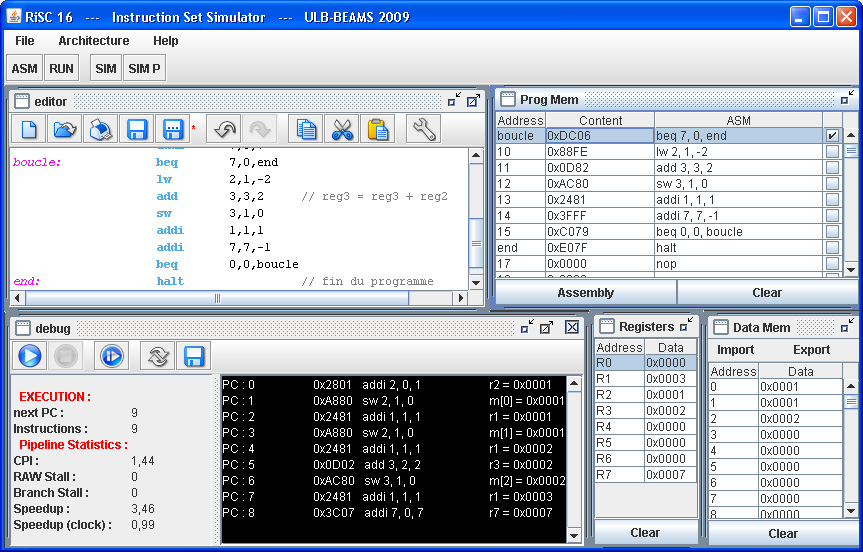
\includegraphics[width=15cm]{100000000000035F000002289D31421E.jpg}
	\end{center}
\caption{Simulator window}
\label{fig:simulator}
\end{figure}

\newpage
\section{Simulator use}
All parameters defining an architecture are available in the menu ``Architecture". Main parameters are:
\begin{itemize}
\item Instruction set (``Architecture > Instruction set"):
\begin{itemize}
\item RiSC16 original: 8 instructions.
\item Special IS[1]: 8 instructions + 8 new instruction. See Table \vref{tab:IS1}.
\item Special IS[2]: same as IS[1] but \verb!BG! replaced by \verb!MUL!.
\item Other: custom instruction set. Instructions can be selected in a list.
\end{itemize}
\item 8, 16, 32 or 64 registers (``Architecture > Registers")
\item Size of immediate constant fields in instructions can be modified (``Architecture > Imm \& Instru size")
\end{itemize}
These parameters will obviously change the instruction length.
%
It is also possible to specify if instructions use signed or unsigned operands. This choice has an impact on \verb!BL! et \verb!BG! and on the way \textit{overflow} and \textit{carry} are processed for instructions \verb!ADD!, \verb!SUB!, \verb!SHL! and  \verb!SHA!.

Several predefined architecture are available in the ``Architecture > preset" menu:
\begin{itemize}
\item Original RiSC16
\item Special IS[1] -- 8 reg -- 16 17-bit instructions, see table \vref{tab:IS1}
\item Special IS[1] -- 16 reg -- 16 24-bit instructions, see table \vref{tab:IS1-16-24}
\item Special IS[2] -- 8 reg -- 16 17-bit instructions, see table \vref{tab:IS2}, \verb!BG! replaced by \verb!MUL!
\end{itemize}

Once the chosen architecture is selected, configured and the assembly code written, the ``RUN" button compiles the program for the selected architecture. New windows will appear to run the actual simulation.

\newpage
\subsection{Assignment}

Compare performances of several algorithm using several instruction sets:

\noindent Choose an operator in $\left\lbrace <, >, \leq, \geq \right\rbrace$.

\begin{Q}
	Determine a set of test vectors which could test the functionality and corner cases of your operator. Justify all vectors utility. We target \textbf{signed numbers}.	[1 point]
\end{Q}

\begin{Q}
	Write the code for your operator using:
	\begin{itemize}
	\item the original 8 instructions [1 point]
	\item the Special IS[1] 17-bit [1 point]
	\end{itemize}
\end{Q}

\begin{Q}

Write a program to multiply the \textbf{unsigned} content of \reg{1} and \reg{2} and write the result in \reg{3} and \reg{4}, LSB in \reg{3}.
\begin{enumerate}
\item Write\footnote{\label{assign}And test it using the online verification tool, the results will be included in the quotation of these labs.} the program using the Special IS[1] 17-bit instruction set. [3 points]
\item Write\footref{assign} the program using the Special IS[2] and using the \verb!MUL! instruction. [3 points]
\item Conclude. [1 point]
\end{enumerate}
Note : the processor uses signed integers (complement to 2 representation) by default.
\end{Q}

\end{document}
